
%✠% \section {Introduction}
\section{简介}

%✠% Let's get you up and running with TensorFlow!
❂本章的目的是让你了解和运行 TensorFlow!

%✠% But before we even get started, let's peek at what TensorFlow code looks like in the Python API, so you have a sense of where we're headed.

❂在开始之前, 让我们先看一段使用 Python API 撰写的 TensorFlow 示例代码,
让你对将要学习的内容有初步的印象.

%✠% Here's a little Python program that makes up some data in two dimensions, and then fits a line to it.

❂下面这段短小的Python程序将把一些数据放入二维空间,再用一条线来拟合这些数据。

\begin{lstlisting}
import tensorflow as tf
import numpy as np

# Create 100 phony x, y data points in NumPy, y = x * 0.1 + 0.3
x_data = np.random.rand(100).astype("float32")
y_data = x_data * 0.1 + 0.3

# Try to find values for W and b that compute y_data = W * x_data + b
# (We know that W should be 0.1 and b 0.3, but Tensorflow will
# figure that out for us.)
W = tf.Variable(tf.random_uniform([1], -1.0, 1.0))
b = tf.Variable(tf.zeros([1]))
y = W * x_data + b

# Minimize the mean squared errors.
loss = tf.reduce_mean(tf.square(y - y_data))
optimizer = tf.train.GradientDescentOptimizer(0.5)
train = optimizer.minimize(loss)

# Before starting, initialize the variables.  We will 'run' this first.
init = tf.initialize_all_variables()

# Launch the graph.
sess = tf.Session()
sess.run(init)

# Fit the line.
for step in xrange(201):
    sess.run(train)
    if step % 20 == 0:
        print(step, sess.run(W), sess.run(b))

# Learns best fit is W: [0.1], b: [0.3]
\end{lstlisting}

%✠% The first part of this code builds the data flow graph. TensorFlow does not actually run any computation until the session is created and the run function is called.

%✠%  To whet your appetite further, we suggest you check out what a classical machine learning problem looks like in TensorFlow. In the land of neural networks the most "classic" classical problem is the MNIST handwritten digit classification. We offer two introductions here, one for machine learning newbies, and one for pros. If you've already trained dozens of MNIST models in other software packages, please take the red pill. If you've never even heard of MNIST, definitely take the blue pill. If you're somewhere in between, we suggest skimming blue, then red.

❂以上代码的第一部分构建了数据的流向图(flow graph)。在一个session被建立并且\lstinline{run()}函数被运行前,TensorFlow不会进行任何实质的计算。

❂为了进一步激发你的学习欲望,我们想让你先看一下TensorFlow是如何解决一个经典的机器学习问题的。在神经网络领域,最为经典的问题莫过于MNIST手写数字分类。为此,我们准备了两篇不同的教程,分别面向初学者和专家。如果你已经使用其它软件训练过许多MNIST模型, 请参阅\hyperref[MINIST_pros]{高级教程(红色药丸)}。如果你以前从未听说过 MNIST, 请先阅读\hyperref[MINIST_beginner]{初级教程(蓝色药丸)}。如果你的水平介于这两类人之间,我们建议你先快速浏览\hyperref[MINIST_beginner]{初级教程}, 然后再阅读\hyperref[MINIST_pros]{高级教程}。

% Add pics and links here.

%✠% If you're already sure you want to learn and install TensorFlow you can skip these and charge ahead. Don't worry, you'll still get to see MNIST -- we'll also use MNIST as an example in our technical tutorial where we elaborate on TensorFlow features.

\begin{center}
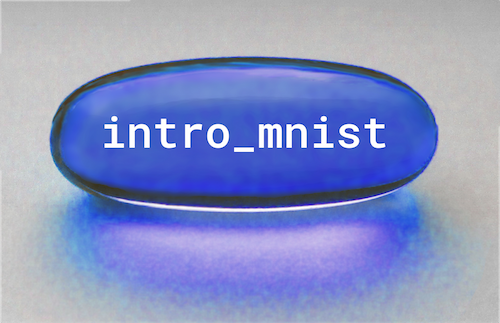
\includegraphics[width=.45\textwidth]{../SOURCE/images/blue_pill.png}

\includegraphics[width=.45\textwidth]{../SOURCE/images/red_pill.png}
\end{center}

❂如果你已下定决心准备学习和安装TensorFlow,你可以略过这些文字,直接阅读
后面的章节\footnote{\textbf{推荐随后阅读内容}:\hyperref[download_install]{1 下载与安装}, \hyperref[basic_usage]{2 基本使用}, \hyperref[tf_mech101]{3 TensorFlow 101}.}。不用担心,你仍然会看到MNIST--在阐述TensorFlow的特性时,
我们还会使用MNIST作为一个样例。


%✠% \textbf{Recommended Next Steps}
%✠%Download and Setup
%✠%Basic Usage
%✠%TensorFlow Mechanics 101


%% \textbf{推荐随后阅读内容}:
%% \begin{itemize}
%% \item \hyperref[download_install]{下载与安装}\\
%% \item \hyperref[basic_usage]{基本使用}\\
%% \item \hyperref[tf_mech101]{TensorFlow 101}\\
%% \end{itemize}